\documentclass[12pt]{article}
\usepackage[utf8]{inputenc}
\usepackage{graphicx}
\usepackage{amsmath} % for mathematical symbols
\usepackage{amssymb} % for \mathbb command
\usepackage[backend=biber,style=numeric]{biblatex}
\graphicspath{ {images/} }
\addbibresource{references.bib} % Specify the name of your .bib file

\title{
{\textbf{Technical University of Košice}}\\
\vspace{12pt}
{\large \textbf{Faculty of Mining, Ecology, Process Control\\ and Geotechnologies}}\\
\vspace{12pt}
{\large Institute of Control and Informatization of Production Processes}\\
\vspace{64pt}
{\textbf{Mathematical method for identification, modelling and simulation}}\\
}
\author{Ing. Ales Jandera}
\date{10. May 2024}

\begin{document}

\maketitle

\newpage

\tableofcontents

\newpage

\section{Basic Concepts}

\textbf{Object}\\
In systems theory, we refer to a real-existing thing as an object, consisting of
interconnected parts.\\
\\
\textbf{System}\\
The object of study. Thus, a system is a certain abstract interpretation of the real
reality - the object. It is a formation consisting of smaller parts (subsystems) that
have mutual connections and also connections to the surroundings of the system.\\
\\
\textbf{Model}\\
Represents the essential properties of real systems in a suitable form, reflecting
information about the system. It expresses or simulates the behavior of the system.\\
\\
\textbf{Model Creation}\\
Models are created based on the relevant equations and conditions. For linear systems,
this involves differential equations; for nonlinear systems, it involves difference
equations.\\
\\
\textbf{Block Description}\\
A graphical representation of the system forms a block, which has one or more inputs
and one or more outputs, and typically includes a relationship between input and output,
most often expressed mathematically (differential equation, image transfer, etc.).
Signals are represented by oriented segments, transformations by blocks, and signal
division by a dot at the junction of the segments.\\
\\
\textbf{Linear Systems}\\
These are systems for which the superposition principle applies, or which have a
linear static characteristic.\\
\\
\textbf{Nonlinear Systems}\\
These are systems where the superposition principle does not apply. Most dynamic
systems are nonlinear. Methods from the field of linear systems do not apply here.\\
\\
\textbf{Static Systems}\\
Systems where, after a step change in the input quantity (action, disturbance), the
output quantity (regulated) stabilizes itself to a new value.\\
\\
\textbf{Dynamic Systems}\\
A formation (thing) with internal organization, exposed to the flow of input signals
(independent of the state and activity of this system) and producing as a result of its
activity a flow of output signals. Time is always an element of the parametric set of a
dynamic system.\\
\\
\textbf{Continuous Systems}\\
Systems whose input, state, and output quantities are defined at any time, i.e.,
there is no time when they are not defined.\\
\\
\textbf{Discrete Systems}\\
Systems where the input, output, and state quantities are defined only at discrete
values of the independent variable. If the system's variables take values from the
set of integers, we say that it is a discrete system.\\
\\
\textbf{Control Objective}\\
The fundamental goal of control is the implementation of automatic control in the
form of automated control systems.\\
\\
\textbf{Approaches}\\
Cybernetic, process-centric / centralized, decentralized\\
\\
\textbf{Method}\\
\begin{itemize}
    \item Feedforward is a method of open-loop control, where the desired value is brought into the control device, which adjusts the control variable according to a given program.
    \item Compensatory is an open control circuit, the desired output value is brought into the compensator, or regulator, which adjusts the control variable of the object also considering the affecting disturbance.
    \item Feedback is closed-loop control, the desired value is compared with the measured actual value, and based on the resulting difference, the regulator adjusts the control variable of the object.
\end{itemize}

\section{Mathematical models}

\subsection{Linear Regression Models}

Linear prediction models are a class of statistical models that assume
 a linear relationship between the input variables and the target
 variable. These models are widely used for prediction and inference
 in various fields such as statistics, machine learning,
 economics, and social sciences.\\
\\
The general form of a linear prediction model can be represented as:\\

\begin{equation}\label{eq1}
    Y = \beta_0 + \beta_1 X_1 + \beta_2 X_2 + \ldots + \beta_p X_p + \epsilon,
\end{equation}

\noindent where\\
\( Y \) is the target variable,\\
\( X_1, X_2, \ldots, X_p \) are the input variables (also known as predictors or features),\\
\( \beta_0, \beta_1, \ldots, \beta_p \) are the coefficients (parameters) representing the strength and direction of the linear relationship between each predictor and the target variable,\\
\( \epsilon \) is the error term representing the difference between the observed and predicted values, assumed to follow a normal distribution with mean zero and constant variance.\\

\noindent Linear prediction models can be categorized into different types based on their
specific characteristics and applications. Some common types of linear prediction models~\cite{WOS:000788587300109, WOS:000426617000001}.\\
\\
\textbf{Simple Linear Regression}\\
A basic linear model with a single predictor variable.\\
\\
\textbf{Multiple Linear Regression}\\
Extends simple linear regression to include multiple predictor variables.\\
\\
\textbf{Generalized Linear Models (GLMs)}\\
A broad class of linear models that allow for non-normal error distributions
and non-linear relationships between predictors and the response variable.\\
\\
\textbf{Ridge Regression and Lasso Regression}\\
Regularized linear regression techniques used for dealing with multicollinearity and
feature selection.\\
\\
Linear prediction models offer several advantages, including interpretability, ease of
implementation, and computational efficiency. However, they also have limitations, such
as the assumption of linearity and the inability to capture complex non-linear
relationships between variables~\cite{WOS:000836807400001}.\\
\\
Despite these limitations, linear prediction models remain a powerful and versatile tool
for predictive modeling and inference in various domains.\\
Linear prediction models, such as linear regression, assume a linear relationship
between the input variables $\mathbf{x}$ and the target variable $y$. Mathematically,
the linear regression model can be expressed as:

\begin{equation}\label{eq2}
    y = \beta_0 + \beta_1 x_1 + \beta_2 x_2 + \ldots + \beta_p x_p + \epsilon,
\end{equation}

\noindent where\\
$y$ is the target variable,\\
$x_1, x_2, \ldots, x_p$ are the input variables (or predictors),\\
$\beta_0, \beta_1, \ldots, \beta_p$ are the coefficients (parameters) representing the slope of the linear relationship between each predictor and the target variable,\\
$\epsilon$ is the error term representing the difference between the actual and predicted values, assumed to be normally distributed with mean zero and constant variance.\\

\noindent The goal of linear regression is to estimate
the coefficients $\beta_0, \beta_1, \ldots, \beta_p$ that minimize the sum of squared
errors (SSE), given a dataset $\{(x_i, y_i)\}_{i=1}^n$. This is typically done using the
method of least squares, where the coefficients are chosen to minimize the sum of the
squared differences between the observed and predicted values:

\begin{equation}
    \hat{\beta} = \arg \min_{\beta} \sum_{i=1}^{n} (y_i - (\beta_0 + \beta_1 x_{i1} + \beta_2 x_{i2} + \ldots + \beta_p x_{ip}))^2
\end{equation}

\noindent Once the coefficients are estimated, the model can be used to predict the target
variable for new observations.\\
\\
\textbf{Simple Linear Regression}\\
\\
Simple Linear Regression is a basic linear prediction model that involves predicting a target
variable \(y\) based on a single predictor variable \(x\). The relationship
between \(x\) and \(y\) is assumed to be linear, and it can be represented by the
equation of a straight line:

\begin{equation}
    y = \beta_0 + \beta_1 x + \epsilon,
\end{equation}

\noindent where\\
\(y\) is the target variable,\\
\(x\) is the predictor variable,\\
\(\beta_0\) is the intercept term, representing the value of \(y\) when \(x\) is zero,\\
\(\beta_1\) is the slope coefficient, representing the change in \(y\) for a one-unit change in \(x\),\\
\(\epsilon\) is the error term, representing the difference between the observed and predicted values, assumed to be normally distributed with mean zero and constant variance.\\

\noindent The goal of Simple Linear Regression is to estimate the parameters \(\beta_0\) and \(\beta_1\) that minimize the sum of squared errors (SSE) between the observed and predicted values of \(y\). This is typically done using the method of least squares, where the coefficients are chosen to minimize the sum of the squared differences between the observed and predicted values:

\begin{equation}
    \hat{\beta_0}, \hat{\beta_1} = \arg \min_{\beta_0, \beta_1} \sum_{i=1}^{n} (y_i - (\beta_0 + \beta_1 x_i))^2
\end{equation}

\noindent Once the coefficients \(\hat{\beta_0}\) and \(\hat{\beta_1}\) are estimated, the
model can be used to predict the target variable \(y\) for new observations based on their
predictor variable \(x\).\\
\\
\textbf{Multiple Linear Regression}\\
Multiple Linear Regression is an extension of Simple Linear Regression that involves predicting a target variable \(y\) based on multiple predictor variables \(x_1, x_2, \ldots, x_p\). The relationship between the predictor variables and the target variable is assumed to be linear, and it can be represented by the equation:

\begin{equation}
    y = \beta_0 + \beta_1 x_1 + \beta_2 x_2 + \ldots + \beta_p x_p + \epsilon,
\end{equation}

\noindent where\\
\(y\) is the target variable,\\
\(x_1, x_2, \ldots, x_p\) are the predictor variables,\\
\(\beta_0\) is the intercept term,\\
\(\beta_1, \beta_2, \ldots, \beta_p\) are the coefficients (parameters) representing the slopes of the linear relationships between each predictor variable and the target variable,\\
\(\epsilon\) is the error term, representing the difference between the observed and predicted values, assumed to be normally distributed with mean zero and constant variance.\\

\noindent The goal of Multiple Linear Regression is to estimate the
parameters \(\beta_0, \beta_1, \ldots, \beta_p\) that minimize the sum of squared
errors (SSE) between the observed and predicted values of \(y\). This is typically done
using the method of least squares, where the coefficients are chosen to minimize the
sum of the squared differences between the observed and predicted Value~\cite{witte2017statistics}:

\begin{equation}
    \hat{\beta_0}, \hat{\beta_1}, \ldots, \hat{\beta_p} = \arg \min_{\beta_0, \beta_1, \ldots, \beta_p} \sum_{i=1}^{n} (y_i - (\beta_0 + \beta_1 x_{i1} + \beta_2 x_{i2} + \ldots + \beta_p x_{ip}))^2
\end{equation}

\noindent Once the coefficients \(\hat{\beta_0}, \hat{\beta_1}, \ldots, \hat{\beta_p}\) are estimated,
the model can be used to predict the target variable \(y\) for new observations based on
their predictor variables \(x_1, x_2, \ldots, x_p\).\\
\\
\textbf{Generalized Linear Models (GLMs)}\\
Generalized Linear Models (GLMs) are a broad class of linear models that extend the linear
regression framework to handle a wider range of response distributions and link functions.
GLMs are particularly useful when the assumptions of normality and constant variance in
linear regression are not met, or when the response variable is not continuous.\\
\\
The general form of a GLM can be expressed as:

\begin{equation}
    g(\mu) = \beta_0 + \beta_1 x_1 + \beta_2 x_2 + \ldots + \beta_p x_p,
\end{equation}

\noindent where\\
\( g(\cdot) \) is the link function,\\
\( \mu \) is the mean of the response variable,\\
\( x_1, x_2, \ldots, x_p \) are the predictor variables,\\
\( \beta_0, \beta_1, \ldots, \beta_p \) are the coefficients (parameters) representing the slopes of the linear relationships between the predictors and the transformed mean.\\

\noindent GLMs consist of three components: 
\begin{enumerate}
    \item \textbf{Random Component}: Specifies the probability distribution of the response variable, which can be any member of the exponential family of distributions, such as normal, binomial, Poisson, gamma, etc.
    \item \textbf{Systematic Component}: Represents the linear combination of predictor variables through the link function.
    \item \textbf{Link Function}: Connects the mean of the response variable to the linear combination of predictors. It allows for modeling non-linear relationships between predictors and the response.
\end{enumerate}

\noindent The parameters of a GLM are estimated using maximum likelihood estimation or iterative weighted
least squares.\\
\\
Once the model is fitted, predictions can be made for new observations using the same
link function and parameter estimates.\\
\\
\textbf{Ridge Regression and Lasso Regression}\\
\\
Ridge Regression and Lasso Regression are regularization techniques used in linear regression
to address multicollinearity and perform feature selection. They add a penalty term to the
ordinary least squares (OLS) cost function to shrink the coefficients towards zero.\\
\\
\textbf{Ridge Regression}\\
\\
Ridge Regression adds a penalty term proportional to the square of the magnitude of the
coefficients (\(\beta\)) to the OLS cost function. The objective function for Ridge Regression
can be expressed as:\\

\begin{equation}
    \text{minimize} \quad J(\beta) = \sum_{i=1}^{n} (y_i - \beta_0 - \sum_{j=1}^{p} \beta_j x_{ij})^2 + \lambda \sum_{j=1}^{p} \beta_j^2,
\end{equation}

\noindent where\\
\(y_i\) is the target variable for the \(i\)th observation,\\
\(x_{ij}\) is the value of the \(j\)th predictor for the \(i\)th observation,\\
\(\beta_0, \beta_1, \ldots, \beta_p\) are the coefficients to be estimated,\\
\(\lambda\) is the regularization parameter that controls the amount of shrinkage.\\

\noindent
\textbf{Lasso Regression}\\
Lasso Regression adds a penalty term proportional to the absolute value of the
magnitude of the coefficients (\(\beta\)) to the OLS cost function. The objective
function for Lasso Regression can be expressed as:\\

\begin{equation}
    \text{minimize} \quad J(\beta) = \sum_{i=1}^{n} (y_i - \beta_0 - \sum_{j=1}^{p} \beta_j x_{ij})^2 + \lambda \sum_{j=1}^{p} |\beta_j|,
\end{equation}

\noindent where\\
\(y_i\) is the target variable for the \(i\)th observation,\\
\(x_{ij}\) is the value of the \(j\)th predictor for the \(i\)th observation,\\
\(\beta_0, \beta_1, \ldots, \beta_p\) are the coefficients to be estimated,\\
\(\lambda\) is the regularization parameter that controls the amount of shrinkage.\\
\\
\noindent Ridge Regression tends to shrink the coefficients towards zero but rarely sets
them exactly to zero, while Lasso Regression can produce sparse models by setting some
coefficients to exactly zero, effectively performing feature selection.\\
\\
The choice between Ridge and Lasso regression depends on the specific characteristics of the dataset and the desired properties of the resulting model.

\subsection{Linear prediction}\label{lp}
Linear prediction is a method, that is extensively employed in signal
processing to forecast future values of a time series by analyzing past observations.
This technique is based on the premise that the current sample of a signal can be described by a linear combination
of previous values complemented by a noise term~\cite{vaidyanathan2007theory,  WOS:000415735500004}. Long-term linear
prediction extends this methodology using not only samples from the current past but also long-term instances, a longer period away, such as months
or years. Although requiring a greater volume of data and increasing the complexity in comparison to
 short-term prediction, its applicability finds use in diverse fields such as weather forecasting, finance, economics and
marketing to make long-term projections about variables such as sales, demand, or stock
prices, with the goal to provide a~comprehensive and accurate forecast that can be used to
make strategic decisions in the~long term~\cite{WOS:A1989AG08300005}.
%
\subsubsection{Short-term linear prediction}\label{slp}
Short-term linear prediction focuses on forecasting the immediate future values in a sequence.
The model representation involves approximating a time series as a linear
combination of its past values, providing a foundation for estimating the next value~\cite{WOS:000836807400001}.
Is a technique commonly used in signal processing and time-series analysis to predict future
values in a sequence based on a linear model.
The basic idea is to use past observations in a sequence to estimate the next value.
Linear prediction is a~statistical technique used to forecast future values based on past
observations. It is a~method for modeling the~relationship between a~dependent variable and
one or more independent variables in a~linear form. The~goal of linear prediction is to find
the~best linear approximation of the relationship between the~variables, which can then be
used to make predictions about future values of the~dependent variable.
%
\subsubsection{Parameters estimation}\label{parameterslp}
Parameter estimation in linear prediction involves determining the coefficients of a linear
model that best represents a given dataset. In the context of linear prediction, this typically
refers to estimating the coefficients of a linear filter that minimizes prediction error.\\
\\
\textbf{Least Squares Estimation}\\
Minimize the sum of squared prediction errors between the model predictions and the actual
observations.\\
\\
\textbf{Maximum Likelihood Estimation}\\
Find the parameters that maximize the likelihood of observing the given data under the assumed
model distribution.\\
\\
\textbf{Yule-Walker Equations}\\
For AR models, the Yule-Walker equations provide a set of linear equations that can be solved
to directly estimate the AR coefficients.\\
\\
\textbf{Burg Algorithm}\\
An iterative algorithm that estimates AR coefficients by minimizing a reflection coefficient
criterion.\\
\\
\textbf{Levinson-Durbin recursion}\\
specific algorithm used for parameter estimation in linear prediction, particularly for
autoregressive (AR) models\\
\\
Assume we have a time series \( x[n] \) that we want to model using an autoregressive model of order \( p \), which can be represented as:
\begin{equation}
     x[n] = \sum_{i=1}^{p} a_i x[n-i] + w[n],
\end{equation}

\noindent where\\
 \( a_i \) are the coefficients of the AR model,\\
\( w[n] \) is white noise, and \( p \) is the order of the model.\\
\\
Toeplitz Matrix Formation arrange the autocorrelation values of the time series into a Toeplitz
matrix \( R \) of size \( (p+1) \times (p+1) \). The \( i \)-th row and \( j \)-th column of this matrix represent
the autocorrelation value at lag \( |i-j| \).\\
\\
The Levinson-Durbin algorithm is a recursive method that efficiently computes the AR
coefficients \( a_i \) using the autocorrelation values stored in the Toeplitz
matrix \( R \). The recursion starts with an initial guess for the first coefficient \( a_1 \) and iteratively
computes the subsequent coefficients using the following steps:
\begin{itemize}
    \item{set \( k = 1 \) and \( E_0 = R[0, 0] \).}
    \item{compute the forward prediction error \( \epsilon_k \) and reflection coefficient \( k_k \) using the formula:
        \begin{equation}
             \epsilon_k = R[k, k] - \sum_{j=1}^{k-1} a_j R[k-j, k] 
        \end{equation}
        \begin{equation}
             k_k = \frac{\epsilon_k}{E_{k-1}}
        \end{equation}}
      \item{update the AR coefficients \( a_k \) using the reflection coefficient \( k_k \):
        \begin{equation}
            a_k = k_k 
        \end{equation}}
      \item{update the prediction error \( E_k \):
        \begin{equation}
             E_k = (1 - k_k^2)E_{k-1} 
        \end{equation}}
      \item{increment \( k \) and repeat the process until all coefficients are computed.}
\end{itemize}
Once all \( p \) coefficients are computed, you obtain the AR model parameters \( a_1, a_2, ..., a_p \).
The Levinson-Durbin recursion provides an efficient way to estimate the parameters of an autoregressive
model by recursively solving linear equations, making it widely used in signal processing,
time series analysis, and speech processing applications.\\
\\
Overall, parameter estimation in linear prediction involves a systematic approach to finding
the coefficients of a linear model that best fits the data and minimizes prediction error.
It requires careful consideration of the model assumptions, choice of estimation method, and
evaluation of model performance.

\subsubsection{Long-term linear prediction} \label{ltlp}
\noindent Long-term linear prediction (LTLP) refers to the~use of linear prediction techniques to make
predictions about the~future values of a~time series over~an~extended period of time~\cite{WOS:000266982600001},
typically several months to several years. Unlike short-term linear prediction, which focuses
on forecasting the~near-term future, long-term linear prediction aims to provide a~more
comprehensive and accurate forecast of future values. Combining these two components, short-term and long-term, one obtains the relation~\cite{vaidyanathan2007theory, WOS:A1990DY40800023}:
%
\begin{equation}\label{eq10}
    \hat{x}(n) = \sum_{i=1}^{p} a_i x(n-i) + \sum_{i=-q}^{q} b_i x(n-i-Q),
\end{equation}
%
where $\hat{x}(n)$ is the~predicted value of the~signal at instance~$n$,
$p$ is the order of the short-term predictor, that uses $p$ past samples, $q$
is the order of the long-term predictor, that uses $2q+1$ samples a pitch period ($Q$) away,
and $a_i$, $b_i$, are the~short-term predictor coefficients, the~long-term predcitor coefficients, respectively (see Fig.~\ref{fig1}).

%
\begin{center}
    \begin{figure}[!ht]
        \centering
        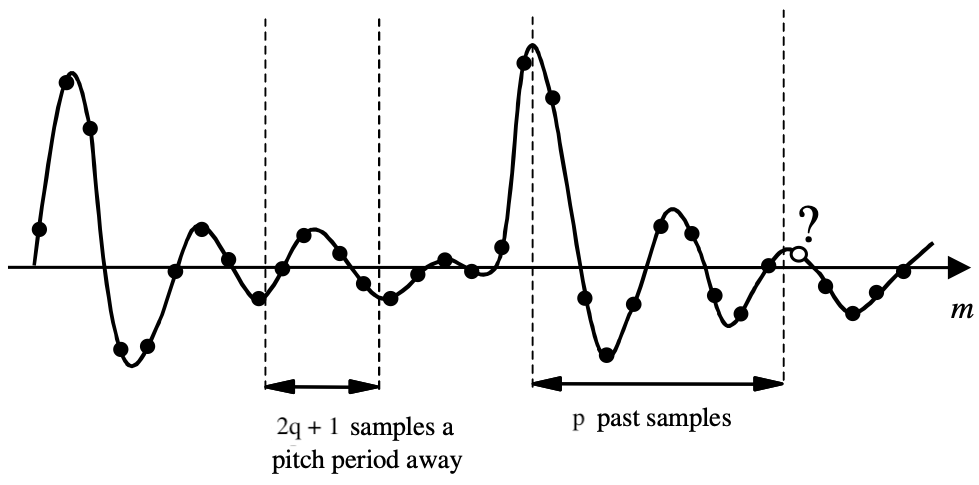
\includegraphics[width=\columnwidth]{shift}
        \caption{Pitch-lag in long-term prediction~\cite{WOS:000266982600001}.}
        \label{fig1}
    \end{figure}
\end{center}

\subsection{Linear Model with Transportation Delay}

A linear model with transportation delay is used to model situationswhe
re there is a linear relationship between input variables and the
output variable, but the output has a time delay caused by the
transportation system or process. This model can be expressed as:\\

\begin{equation}
    y(t) = \beta_0 + \beta_1 x(t - \tau) + \epsilon,
\end{equation}

\noindent where\\
\( y(t) \) is the output variable at time \( t \),\\
\( x(t - \tau) \) is the input variable at time \( t - \tau \), where \( \tau \) is the transportation delay,\\
\( \beta_0 \) and \( \beta_1 \) are the coefficients of the model,\\
\( \epsilon \) is the model error.\\

\noindent This model is used, for example, in modeling signals in telecommunications
or in modeling dynamic systems with time delays.

\subsection{Non-linear Models}

Nonlinear prediction models are mathematical frameworks used to capture complex relationships
between input variables and the target variable in prediction tasks. Unlike linear models,
which assume a linear relationship between predictors and the target, nonlinear models can
capture more intricate patterns in the data. Here's an overview of some common nonlinear
prediction models~\cite{WOS:000980444400020}.\\
\\
\subsubsection{Volterra Series}
The Volterra series~\cite{wiener1958} models the output of a nonlinear system as a functional series,
where the output depends not only on the current input but also on past inputs, capturing
the history-dependent behavior of the system. This is crucial for accurately describing
systems where the output is not merely a direct proportional response to the input.\\
\\
Components of the Volterra Series:\\
\begin{enumerate}
\item Linear and Nonlinear Kernels of the Volterra series is built up of kernels of
increasing order that correspond to the system's linear, quadratic, cubic, and
higher-order responses. Each kernel integrates the product of input values at multiple
time points, reflecting the combined effects of these inputs over time.
\item Integration over Time Delays involve the kernels integration over different combinations
of time delays, representing how past inputs influence the current output.
This integration makes the model particularly useful for analyzing systems with memory.\\
\item Expansion Terms series includes terms of increasing complexity, with each
higher-order term accounting for more complex interactions between input values
at different times. The first-order kernel represents the linear response, the
second-order kernel captures pairwise interactions (quadratic nonlinearity), and
higher-order kernels describe more complex dynamics.
\end{enumerate}

\noindent Applications of Voltera Series models are in the \textbf{Signal Processing} where Volterra series
are used to model and predict nonlinear distortions in signals, such as
in audio processing or telecommunications, where equipment nonlinearity affects the
signal integrity then in \textbf{Control Systems} in control theory helps in designing controllers
that can handle nonlinear dynamics effectively, ensuring stability and performance in
nonlinear control systems. In the \textbf{Biological Systems} are applied in modeling
the nonlinear responses of biological systems, such as the neural response functions
in sensory systems where the output response to stimuli is inherently nonlinear.\\
\\
As the order of interaction increases, the computational complexity of the model can
grow significantly, making higher-order models difficult to manage. Accurately estimating
the higher-order kernels requires extensive data, and the model may suffer from
overfitting if not properly regularized or if the data is not sufficient.\\
\\
The Volterra series provides a powerful framework for understanding and predicting
the behavior of nonlinear systems, though its practical application requires careful
consideration of its complexity and the computational resources available.\\
\\
\textbf{Volterra Series Expansion}\\
\\
The output \( y(t) \) of a nonlinear system in response to an input \( x(t) \) can be
expressed as:
\begin{equation}
    y(t) = h_0 + \sum_{n=1}^{\infty} \int_{-\infty}^\infty \int_{-\infty}^\infty \cdots \int_{-\infty}^\infty h_n(\tau_1, \tau_2, \ldots, \tau_n) x(t-\tau_1) x(t-\tau_2) \cdots x(t-\tau_n) \, d\tau_1 \, d\tau_2 \cdots d\tau_n,
\end{equation}
\noindent where, \( h_n(\tau_1, \tau_2, \ldots, \tau_n) \) are the Volterra kernels, which
are functions characterizing the system's response at different orders of interaction
between time-shifted inputs. Each kernel \( h_n \) corresponds to the \( n \)-th order
of nonlinearity in the system's response:\\

\noindent \( h_0 \) is a constant term, often representing the system's output at zero input.
\( h_1(\tau_1) \) is the first-order kernel or linear response of the system.
\( h_2(\tau_1, \tau_2) \) is the second-order kernel, capturing the pairwise nonlinear interactions.
\( h_3(\tau_1, \tau_2, \tau_3) \)* and higher-order kernels account for increasingly complex interactions.\\
\\
\textbf{First and Second-Order Kernels}\\
\\
For practical applications, the Volterra series is often truncated after a few terms.
Here's how the first and second-order terms are typically expressed:\\
\\
First-order (linear) response:\\
\begin{equation}
   y_1(t) = \int_{-\infty}^\infty h_1(\tau_1) x(t-\tau_1) \, d\tau_1
\end{equation}

Second-order (quadratic) response:\\
\begin{equation}
    y_2(t) = \int_{-\infty}^\infty \int_{-\infty}^\infty h_2(\tau_1, \tau_2) x(t-\tau_1) x(t-\tau_2) \, d\tau_1 \, d\tau_2
\end{equation}
\\
\subsubsection{Polynomial Regression}
Polynomial regression is a form of regression analysis in which the relationship between
the independent variable \(x\) and the dependent variable \(y\) is modeled as an nth degree
polynomial. Polynomial regression fits a nonlinear relationship between the value
of \(x\) and the corresponding conditional mean of \(y\), denoted \(E(y|x)\). Although
the model is nonlinear in the predictors, it is linear in the parameters, making it a
form of linear regression.\\
\\Polynomial regression can fit a wide range of curvature in the data by adjusting
the degree of the polynomial, providing a better fit to the dataset than simple
linear regression.\\
\\
\textbf{Degree of Polynomial}\\
The degree of the polynomial is a crucial choice in polynomial regression. Higher degrees
can fit the data better but can also lead to overfitting where the model captures noise
rather than the underlying data pattern. Typically, polynomial terms up to the second
degree (quadratic), third degree (cubic), or fourth degree are used, depending on the data
complexity.\\
\\
\textbf{Model Equation}
\begin{equation}
   y = \beta_0 + \beta_1x + \beta_2x^2 + \beta_3x^3 + ... + \beta_nx^n + \epsilon.
\end{equation}
where \( \beta_0, \beta_1, ..., \beta_n \) are parameters to be estimated,
and \( \epsilon \) is the error term.\\
\\
Polynomial regression is widely used in situations where data exhibit trends that are
not captured well by linear models. This includes fields like economics for trend
analysis, in science for empirical formulas based on experimental data, and in quality.

\subsubsection{Generalized Additive Models (GAMs)}
Generalized Additive Models (GAMs) are a flexible class of models used in statistics to
extend linear models by allowing non-linear functions of the predictor variables while
maintaining overall interpretability. Developed by Trevor Hastie and Robert Tibshirani in
the late 1980s, GAMs provide a way to model complex behaviors in data without specifying
a parametric form for the relationship between predictors and response variable.\\
\\
GAMs generalize the linear model by allowing the linear predictor to depend linearly on
unknown smooth functions of some predictor variables. The general form of a GAM is:
\begin{equation}
   g(E(Y)) = \beta_0 + f_1(X_1) + f_2(X_2) + \ldots + f_p(X_p),
\end{equation}
where, \( g \) is a link function (as used in Generalized Linear
Models, GLMs), \( E(Y) \) is the expected value of the response
variable \( Y \), \( \beta_0 \) is the intercept, and \( f_i \) are smooth,
non-linear functions of the predictor variables \( X_i \).\\
\\
The functions \( f_i(X_i) \) can be specified in various ways, typically using splines
or local regression techniques. This allows the model to capture complex nonlinear
relationships between each predictor and the response.Each function \( f_i \) is
estimated from the data, typically through a backfitting algorithm that iteratively
updates each function to better fit the data while keeping other functions fixed.\\
\\
GAMs are particularly useful in scenarios where the relationship between the response and
predictors is suspected to be non-linear or involves interactions, such as in ecological
modeling, epidemiology, and economic forecasting.\\
They are used in both regression (continuous response) and classification (categorical
response) contexts. GAMs can model complex patterns in the data without assuming a specific
parametric form for the relationship. They can handle varying types of data and
distributions by choosing an appropriate link function and error distribution, much like
GLMs.\\
\subsubsection{Neural Networks}
Neural networks are inspired by the neural architecture of the human brain,
consisting of interconnected neurons organized
into layers. These networks process raw data from the input layer through hidden layers,
which perform computations and adjust weights to yield predictions. Ultimately, the output
layer provides the final result in the form of parameter prediction or classification~\cite{WOS:001091632800001}.
%
Neural networks are trained on large datasets using a~process called backpropagation, which
adjusts the~weights and biases of the~neurons to minimise the~error between the~predicted output
and the~actual output. Once a~neural network has been trained, it can be used to make predictions
on new data~\cite{WOS:000659928700099}.\\
\\
An~artificial neuron or a~perceptron (Fig.~\ref{fig:perceptron}) is a~basic building block
of a~neural network, that is modelled based on the~biological neurons in the~human brain,
that receive input signals from other neurons, process them, and send the output signals to
other neurons.
%
\begin{center}
    \begin{figure}[!ht]
        \centering
        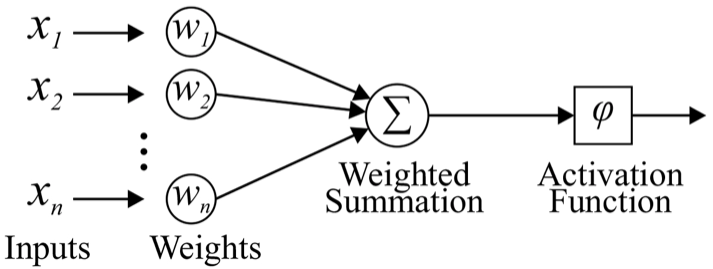
\includegraphics[width=0.8\columnwidth]{nn}
        \caption{Perceptron preview \cite{WOS:000466708200028}.}
        \label{fig:perceptron}
    \end{figure}
\end{center}
Each input $x_n$ undergoes weighting by the
corresponding weight $w_n$ before entering the summation stage. Subsequently, the weighted
summation is transmitted to the activation unit, which generates the neuron's output signal.\\
\\
\subsubsection{Gaussian Processes}
Gaussian processes are probabilistic models that represent distributions over functions.
They are particularly useful for modeling uncertainty and can capture complex nonlinear
patterns in the data.\\
\\
These nonlinear prediction models offer flexibility in capturing intricate relationships
in the data and are widely used in various fields such as finance, healthcare, engineering,
and more. Choosing the appropriate model depends on the specific characteristics of the
data and the task at hand.\\
\\
\textbf{Gaussian Process Regression}\\
\\
At the core of Gaussian process regression (GPR), the idea is that the data can be
described by a Gaussian distribution characterized by a mean and a covariance
function (or kernel). This approach assumes that the function values are random
variables which have a joint Gaussian distribution.\\
\\
The fundamental equation for a Gaussian Process is generally expressed as:
\begin{equation}
    y(x) = f(x) + \epsilon,
\end{equation}
Where:
\( y(x) \) is the observed output at point \( x \),
\( f(x) \) is the latent function that we want to learn,
\( \epsilon \) is the noise in the observations, typically assumed to be Gaussian, i.e., \( \epsilon \sim \mathcal{N}(0, \sigma^2) \).\\
\newpage
\noindent \textbf{Gaussian Process Model}\\
\\
A Gaussian process is fully specified by its mean function \( m(x) \) and covariance
function \( k(x, x') \):
\begin{equation}
    f(x) \sim \mathcal{GP}(m(x), k(x, x')),
\end{equation}
Where:
\( m(x) \) is the mean function, which is often assumed to be zero in many applications because the GP can model the mean arbitrarily well with enough data.
\( k(x, x') \) is the covariance function or kernel, which defines the shape of the function or the way in which the function values are correlated with each other. Popular choices for the kernel include the Squared Exponential (SE), Rational Quadratic, or Matérn kernels.\\
\\
\textbf{Predictive Distribution}\\
\\
Given some observed data points \( D = \{(x_i, y_i)\}_{i=1}^n \) and a new test
point \( x^* \), the predictive distribution of the output \( y^* \) at \( x^* \) is also
Gaussian:
\begin{equation}
    y^*|x^*, D \sim \mathcal{N}(\mu^*, \sigma^{*2})
\end{equation}
With the predictive mean and variance given by:\\
\begin{equation}
\mu^* = k(x^*, X) [K + \sigma^2I]^{-1} Y
\end{equation}
\begin{equation}
\sigma^{*2} = k(x^*, x^*) - k(x^*, X) [K + \sigma^2I]^{-1} k(X, x^*),
\end{equation}
where:\\
\( X \) is the matrix of training inputs,\\
\( Y \) is the vector of training outputs,\\
\( K \) is the covariance matrix computed between all pairs of training inputs,\\
\( k(x^*, X) \) is the vector of covariances between the test point and all training points,\\
\( k(x^*, x^*) \) is the variance of the test point under the GP prior,\\
\( I \) is the identity matrix,\\
\( \sigma^2 \) is the noise variance.

\subsection{Non-linear Model with Transportation Delay}

A nonlinear model with transportation delay extends the linear model by
allowing nonlinear relationships between input and output variables and
also includes time delay caused by the transportation system. This model
can be generally expressed as:

\begin{equation}
    y(t) = f(x(t - \tau), \theta) + \epsilon,
\end{equation}

\noindent where:\\
\( y(t) \) is the output variable at time \( t \),\\
\( f \) is a nonlinear function,\\
\( \tau \) is the transportation delay\\
\( \theta \) are the parameters of the nonlinear model,\\
\( \epsilon \) is the model error.\\

\noindent Non-linear models with transportation delay are used in various fields,
including biology, economics, and engineering, where it is important to
model complex dynamic systems with time delays and nonlinearities. 
These models can better capture reality and provide more accurate
predictions than linear models.

\section{Behavioral models}
Behavioral model are based on several different theories which
simulates the behavioral systems.\\
\subsection{Game Theory}\label{gt}
Game theory is a mathematical framework for analyzing strategic
interactions between rational decision-makers. It models situations where
the outcome of one agent's actions depends on the actions of others.
Game theory is used to study various aspects of human behavior, including
cooperation, competition, bargaining, and negotiation.\\
\\
Mathematical overview of Game Theory:\\
\\
\textbf{Players}\\
In a game, there are \(n\) players, denoted by \(N = \{1, 2, \ldots, n\}\).\\
\\
\textbf{Strategies}\\
Each player \(i\) has a set of strategies \(S_i\), representing all possible actions or choices available to that player. A strategy \(s_i\) for player \(i\) is an element of \(S_i\), and a strategy profile \(s = (s_1, s_2, \ldots, s_n)\) represents a complete set of strategies chosen by all players.\\
\\
\textbf{Payoffs}\\
The payoff function \(u_i : S_1 \times S_2 \times \ldots \times S_n \rightarrow \mathbb{R}\) specifies the utility or payoff that player \(i\) receives for choosing strategy \(s_i\) given that the other players choose strategies \(s_{-i} = (s_1, s_2, \ldots, s_{i-1}, s_{i+1}, \ldots, s_n)\). Mathematically, it can be written as:\\
\begin{equation}
    u_i(s_1, s_2, \ldots, s_n)
\end{equation}

\noindent \textbf{Equilibrium Concepts}\\
\begin{enumerate}
\item Nash Equilibrium (NE)
A strategy profile \(s^* = (s_1^*, s_2^*, \ldots, s_n^*)\) is a Nash equilibrium if, for each player \(i\), their strategy \(s_i^*\) maximizes their payoff given the strategies chosen by the other players \(s_{-i}^*\). Mathematically, for each player \(i\), we have:

\begin{equation}
 u_i(s_i^*, s_{-i}^*) \geq u_i(s_i, s_{-i}^*) \quad \forall s_i \in S_i 
\end{equation}
\item Subgame Perfect Equilibrium (SPE)
In dynamic games, a strategy profile \(s^*\) is a subgame perfect equilibrium if it represents a Nash equilibrium in every subgame of the original game. This ensures that each player's strategy is optimal not only in the current stage but also in every possible future stage of the game.

\item Bayesian Nash Equilibrium (BNE)
In games with incomplete information, where players have private information, a strategy profile \(s^*\) is a Bayesian Nash equilibrium if, for each player \(i\), their strategy \(s_i^*\) maximizes their expected payoff given their beliefs about the other players' types or characteristics.
\end{enumerate}

\noindent These equations provide the mathematical foundation for analyzing strategic interactions in Game Theory, enabling the identification of stable outcomes and predicting the behavior of rational decision-makers in various contexts.

\subsection{Utility Theory}\label{ut}
Utility theory is a mathematical framework for representing and analyzing
individual preferences and decision-making under uncertainty. It assumes
that individuals make decisions to maximize their utility, where utility
represents the subjective value or satisfaction derived from different
outcomes. Utility theory is often used in economics and decision theory
to model and predict human behavior.\\
\\
Utility theory is a branch of economics that deals with how individuals make choices
based on their preferences and the trade-offs they face. The fundamental concept
in utility theory is the notion of utility, which represents the satisfaction or 
appiness a person derives from consuming a good or experiencing an outcome.\\
\\
\textbf{Utility Function}\\
A utility function, typically denoted by \( U(x) \), maps consumption bundles
(combinations of goods or outcomes) to a numerical representation of the utility or
satisfaction derived from consuming that bundle. Mathematically, it can be represented as:\\

\begin{equation}
    U(x_1, x_2, ..., x_n),
\end{equation}

\noindent where\\
 \( x_1, x_2, ..., x_n \) are the quantities of different goods or outcomes in the
consumption bundle.\\
\\
\textbf{Total Utility}\\
Total utility is the overall level of satisfaction or happiness obtained from
consuming a particular set of goods or experiencing a particular outcome.
It is the sum of the utilities derived from each individual good or outcome.\\

\begin{equation}
    TU = U(x_1) + U(x_2) + ... + U(x_n)
\end{equation}
\\
\textbf{Marginal Utility}\\
Marginal utility represents the additional utility obtained from consuming one
additional unit of a good or experiencing one additional unit of an outcome,
while holding the consumption of other goods constant. Mathematically, it is
the derivative of the utility function with respect to the quantity of the good:\\

\begin{equation}
    MU = \frac{dU}{dx},
\end{equation}

\noindent where\\
\( MU \) is the marginal utility,\\
\( dx \) is a small change in the quantity of the good.\\
\\
\textbf{Diminishing Marginal Utility}\\
This principle states that as a person consumes more of a good, the additional
satisfaction (or marginal utility) derived from each additional unit of the good decreases.
Mathematically, it implies that the marginal utility function is decreasing:

\begin{equation}
    \frac{d^2U}{dx^2} < 0
\end{equation}

\noindent These are some of the fundamental equations and concepts in utility theory.
They help economists and decision-makers understand how individuals make choices based
on their preferences and constraints.

\subsection{Bayesian Decision Theory}\label{bt}
Bayesian decision theory is a mathematical framework for decision-making
under uncertainty, based on the principles of Bayesian probability theory.
It models decisions as choices among possible actions, where each action
has associated uncertain outcomes and probabilities. Bayesian decision
theory provides a formal method for incorporating prior beliefs and
updating them based on new evidence to make optimal decisions.\\
\\
\textbf{Prior Probability}\\
Before observing any data, we have beliefs about the likelihood of different events
occurring. This is represented by the prior probability
distribution \( P(\theta) \), where \( \theta \) is a parameter representing the uncertain
quantity.\\
\\
\textbf{Likelihood Function}\\
Given a particular value of the parameter \( \theta \), the likelihood
function \( L(\theta | x) \) describes the probability of observing
the data \( x \). It represents how well the data supports different
values of the parameter.\\
\\
\textbf{Posterior Probability}\\
After observing the data \( x \), we update our beliefs about the
parameter \( \theta \) using Bayes' theorem:\\

\begin{equation}
    P(\theta | x) = \frac{L(\theta | x) \cdot P(\theta)}{P(x)},
\end{equation}

\noindent where\\
\( P(\theta | x) \) is the posterior probability distribution, representing our updated beliefs about \( \theta \) after observing the data \( x \),\\
\( P(x) \) is the marginal likelihood or evidence, which acts as a normalization constant and ensures that the posterior distribution integrates to 1.\\
\\
\textbf{Decision Rule}\\
A decision rule specifies how to choose an action based on the observed data and the
posterior distribution. The decision rule could be to choose the action that maximizes
expected utility.\\
\\
\noindent \textbf{Expected Utility}\\
The expected utility of taking action \( a \) given the observed data is calculated
as the weighted average of the utility of each possible outcome, where the weights
are the probabilities of those outcomes given the data:\\

\begin{equation}
    EU(a | x) = \sum_{\theta} P(\theta | x) \cdot U(a, \theta),
\end{equation}

\noindent where\\
\( EU(a | x) \) is the expected utility of action \( a \) given the data \( x \),\\
\( U(a, \theta) \) is the utility of taking action \( a \) under parameter \( \theta \).\\
\\
\textbf{Decision Theory Loss Function}\\
Decision theory often involves defining a loss function \( L(a, \theta) \) that quantifies
the cost or loss associated with taking action \( a \) when the true parameter
is \( \theta \). The goal is to minimize the expected loss.\\
\\
These equations and concepts provide a framework for making decisions under uncertainty
in a principled and rational manner, incorporating both prior beliefs and observed data.

\subsection{Stochastic Models}\label{sm}
Stochastic models are mathematical models that incorporate randomness or
uncertainty into the modeling of human behavior. These models often use
probability distributions to describe random variables and stochastic
processes to model the evolution of these variables over time. Stochastic
models are used to study various phenomena in human behavior, including
risk-taking, decision-making under uncertainty, and the dynamics of social
systems.\\
\\
\textbf{Stochastic Process}\\
A stochastic process is a collection of random variables indexed by time or some other
parameter. Mathematically, it is represented as \( X(t) \), where \( t \) is the time parameter.\\
\\
\noindent \textbf{Probability Distribution}\\
Stochastic models often involve probability distributions to describe the uncertainty
associated with random variables. Common probability distributions include:\\
\begin{itemize}
   \item Normal (Gaussian) distribution
   \item Poisson distribution
   \item Exponential distribution
   \item Binomial distribution
   \item Multinomial distribution
   \item Geometric distribution
\end{itemize}
\noindent \textbf{Markov Chains}\\
Markov chains are stochastic processes with the Markov property, which states that the future
behavior of the process depends only on its current state and not on its past history.
Mathematically, for a discrete-time Markov chain with states \( S \) and transition
probabilities \( P \), the Markov property is represented as:\\
\begin{equation}
    P(X_{n+1} = j | X_n = i, X_{n-1} = i_{n-1}, ..., X_0 = i_0) = P(X_{n+1} = j | X_n = i)
\end{equation}
\\
\textbf{Continuous-Time Markov Chains (CTMC)}\\
CTMCs are Markov chains where time is continuous. The transition rates between
states are constant and independent of time. The master equation governs the evolution
of the probability distribution of states over time in a CTMC.\\
\\
\textbf{Stochastic Differential Equations (SDEs)}\\
SDEs describe the evolution of a stochastic process over continuous time.
They are differential equations that involve both deterministic and stochastic components.
A simple form of SDE is given by:\\
\\
\begin{equation}
    dX(t) = \mu(X(t), t) \, dt + \sigma(X(t), t) \, dW(t),
\end{equation}
where\\
\( X(t) \) is the stochastic process,\\
\( \mu(X(t), t) \) represents the deterministic drift term,\\
\( \sigma(X(t), t) \) represents the stochastic diffusion term,\\
\( dW(t) \) is a Wiener process (Brownian motion), representing random fluctuations.\\
\\
\textbf{Ito's Lemma}\\
Ito's Lemma is a formula used to find the differential of a function of a stochastic
process. It extends the chain rule to include stochastic terms.
For a function \( f(X(t), t) \) of a stochastic process \( X(t) \), Ito's Lemma is given by:\\

\begin{equation}
    df(X(t), t) = \frac{\partial f}{\partial t} \, dt + \frac{\partial f}{\partial x} \, dX(t) + \frac{1}{2} \frac{\partial^2 f}{\partial x^2} \, (\sigma(X(t), t))^2 \, dt
\end{equation}

\noindent These equations and concepts form the foundation of stochastic modeling and are used to
describe and analyze systems subject to randomness or uncertainty.

\subsection{Network Models}\label{nm}
Network models are mathematical representations of social or relational
structures, where nodes represent individuals or entities, and edges
represent relationships or interactions between them. These models are
used to study various aspects of human behavior, including social influence,
information diffusion, and the spread of behaviors or diseases through
social networks. Network analysis techniques, such as centrality measures
and community detection algorithms, are used to analyze and interpret network data.\\
\\
\textbf{Graph Theory}\\
Network models are often described using graph theory,
where a graph \( G = (V, E) \) consists of a set of
vertices (nodes) \( V \) and a set of edges \( E \) that connect pairs
of vertices. Mathematically, a graph can be represented as an adjacency
matrix, \( A \), where \( A_{ij} = 1 \) if there is an edge between
nodes \( i \) and \( j \), and \( A_{ij} = 0 \) otherwise~\cite{bondy2008graph, WOS:000988346000001}.\\
\\
\textbf{Degree Distribution}\\
The degree of a node in a network is the number of edges incident to it.
The degree distribution \( P(k) \) gives the probability that a randomly chosen node
has degree \( k \). It can be characterized using mathematical functions such as power-law
distributions, exponential distributions, or Poisson distributions.\\
\\
\textbf{Centrality Measures}\\
Centrality measures quantify the importance of nodes within a network.
Some common centrality measures include \textbf{Degree centrality} as the number of edges
incident to a node. \textbf{Betweenness centrality} as the fraction of shortest paths that
pass through a node. \textbf{Eigenvector centrality} as the influence of a node in the network,
taking into account the centrality of its neighbors.\\
\\
\textbf{Random Graph Models}\\
Random graph models are used to generate synthetic networks with specific structural
properties. Examples include:\\
\begin{itemize}
   \item Erdős-Rényi model: A random graph where each edge is present with a fixed probability.
   \item Barabási-Albert model: A preferential attachment model where new nodes are connected to existing nodes with probability proportional to their degree.
   \item Watts-Strogatz model: A small-world model where most nodes are connected to their nearest neighbors, with a small probability of rewiring edges to create shortcuts.
\end{itemize}

\noindent \textbf{Network Dynamics}\\
Network models can capture the dynamics of processes that unfold on networks. For example 
\textbf{Epidemic models}, which describe the spread of diseases or information
through a network. \textbf{Diffusion models} to study the adoption of innovations or behaviors
among individuals in a social network. \textbf{Opinion dynamics} to explore how opinions or
beliefs evolve within a population through interactions on a network.\\
\\
\textbf{Network Optimization}\\
In various applications, network models are used to optimize certain objectives subject to
constraints. Optimization problems on networks can be formulated using mathematical
programming techniques, such as linear programming, integer programming, or network
flow algorithms.\\
\\
These mathematical equations and concepts provide a foundation for analyzing and understanding
the structure, function, and dynamics of complex networks in diverse fields.
\newpage
\printbibliography
\end{document}